\begin{figure}[h!t]
	\centering
        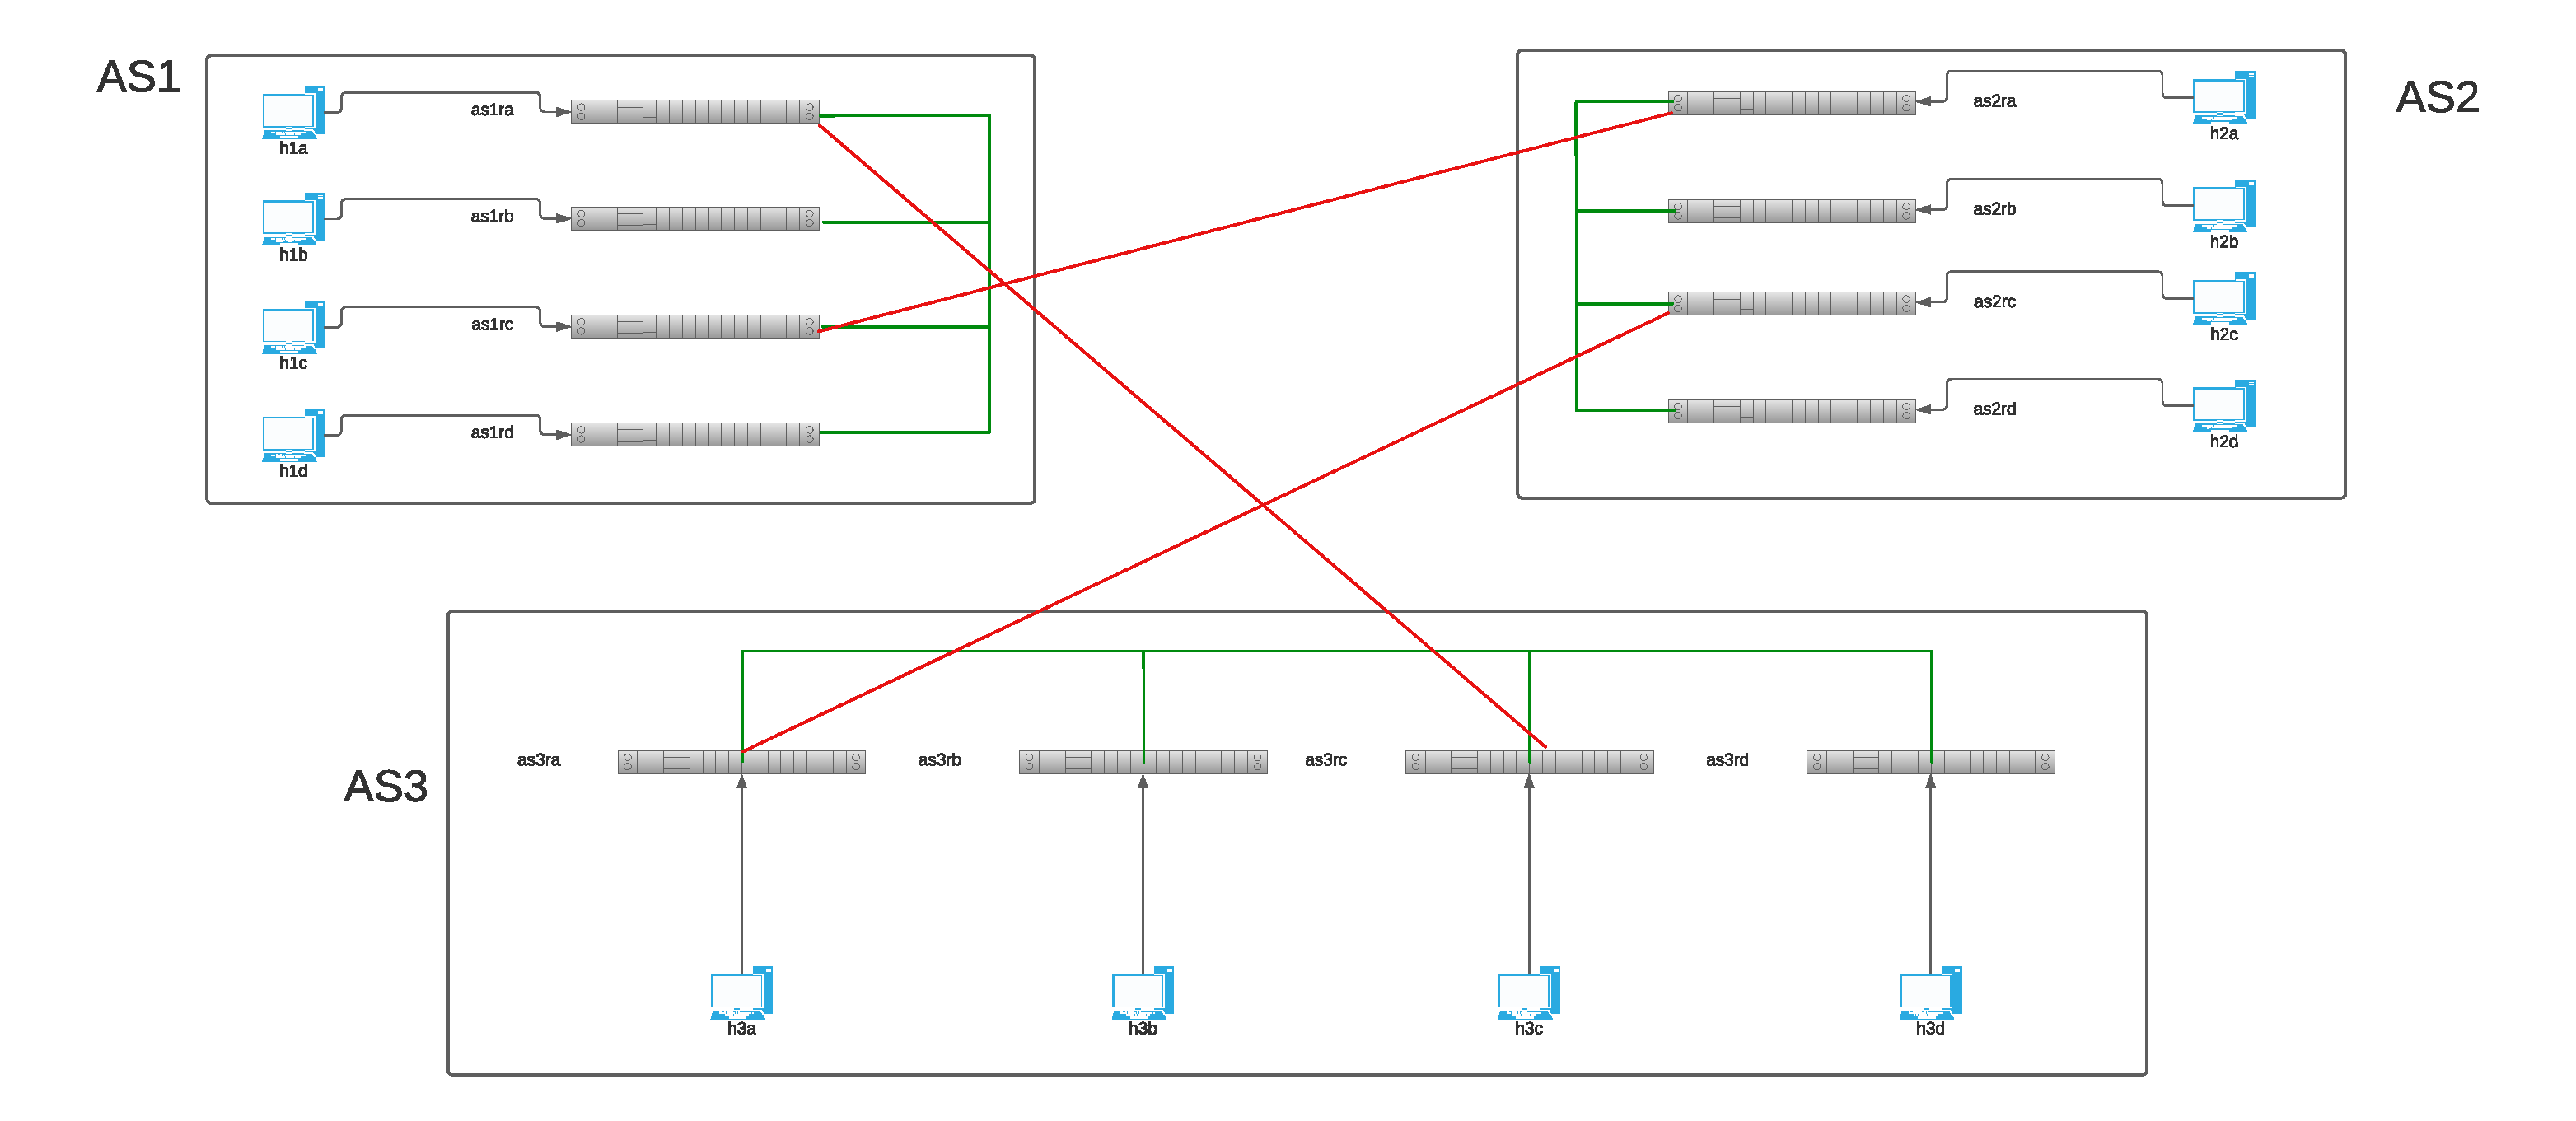
\includegraphics[width=\linewidth]{graphics/diagram.pdf}	
        \caption{Network configuration}
\end{figure}
\begin{table}[h!]
\centering
\begin{tabular}{|c|c|c|}
\hline
\textbf{Node} & \textbf{Interface Name} & \textbf{IP Address} \\
\hline
as1ra & as1ra-h1a & fc00:0:1:a::a/64 \\
h1a & h1a-as1ra & fc00:0:1:a::1/64 \\

as1rb & as1rb-h1b & fc00:0:1:b::b/64 \\
h1b & h1b-as1rb & fc00:0:1:b::1/64 \\

as1rc & as1rc-h1c & fc00:0:1:c::c/64 \\
h1c & h1c-as1rc & fc00:0:1:c::1/64 \\

as1rd & as1rd-h1d & fc00:0:1:d::d/64 \\
h1d & h1d-as1rd & fc00:0:1:d::1/64 \\

as2ra & as2ra-h2a & fc00:0:2:a::a/64 \\
h2a & h2a-as2ra & fc00:0:2:a::2/64 \\

as2rb & as2rb-h2b & fc00:0:2:b::b/64 \\
h2b & h2b-as2rb & fc00:0:2:b::2/64 \\

as2rc & as2rc-h2c & fc00:0:2:c::c/64 \\
h2c & h2c-as2rc & fc00:0:2:c::2/64 \\

as2rd & as2rd-h2d & fc00:0:2:d::d/64 \\
h2d & h2d-as2rd & fc00:0:2:d::2/64 \\

as3ra & as3ra-h3a & fc00:0:3:a::a/64 \\
h3a & h3a-as3ra & fc00:0:3:a::3/64 \\

as3rb & as3rb-h3b & fc00:0:3:b::b/64 \\
h3b & h3b-as3rb & fc00:0:3:b::3/64 \\

as3rc & as3rc-h3c & fc00:0:3:c::c/64 \\
h3c & h3c-as3rc & fc00:0:3:c::3/64 \\

as3rd & as3rd-h3d & fc00:0:3:d::d/64 \\
h3d & h3d-as3rd & fc00:0:3:d::3/64 \\
\hline
\end{tabular}
\caption{IP addresses for hosts attached to routers}
\label{table:gbp_interfaces}
\end{table}
\begin{table}[h!]
\centering
\begin{tabular}{|c|c|c|}
\hline
\textbf{Node} & \textbf{Interface Name} & \textbf{IP Address} \\
\hline
as1ra & as1ra-as1rb & fc00:0:1:ab::a/64 \\
as1rb & as1rb-as1ra & fc00:0:1:ab::b/64 \\

as1ra & as1ra-as1rc & fc00:0:1:ac::a/64 \\
as1rc & as1rc-as1ra & fc00:0:1:ac::c/64 \\

as1ra & as1ra-as1rd & fc00:0:1:ad::a/64 \\
as1rd & as1rd-as1ra & fc00:0:1:ad::d/64 \\

as1rb & as1rb-as1rc & fc00:0:1:bc::b/64 \\
as1rc & as1rc-as1rb & fc00:0:1:bc::c/64 \\

as1rb & as1rb-as1rd & fc00:0:1:bd::b/64 \\
as1rd & as1rd-as1rb & fc00:0:1:bd::d/64 \\

as1rc & as1rc-as1rd & fc00:0:1:cd::c/64 \\
as1rd & as1rd-as1rc & fc00:0:1:cd::d/64 \\

as2ra & as2ra-as2rb & fc00:0:2:ab::a/64 \\
as2rb & as2rb-as2ra & fc00:0:2:ab::b/64 \\

as2ra & as2ra-as2rc & fc00:0:2:ac::a/64 \\
as2rc & as2rc-as2ra & fc00:0:2:ac::c/64 \\

as2ra & as2ra-as2rd & fc00:0:2:ad::a/64 \\
as2rd & as2rd-as2ra & fc00:0:2:ad::d/64 \\

as2rb & as2rb-as2rc & fc00:0:2:bc::b/64 \\
as2rc & as2rc-as2rb & fc00:0:2:bc::c/64 \\

as2rb & as2rb-as2rd & fc00:0:2:bd::b/64 \\
as2rd & as2rd-as2rb & fc00:0:2:bd::d/64 \\

as2rc & as2rc-as2rd & fc00:0:2:cd::c/64 \\
as2rd & as2rd-as2rc & fc00:0:2:cd::d/64 \\

as3ra & as3ra-as3rb & fc00:0:3:ab::a/64 \\
as3rb & as3rb-as3ra & fc00:0:3:ab::b/64 \\

as3ra & as3ra-as3rc & fc00:0:3:ac::a/64 \\
as3rc & as3rc-as3ra & fc00:0:3:ac::c/64 \\

as3ra & as3ra-as3rd & fc00:0:3:ad::a/64 \\
as3rd & as3rd-as3ra & fc00:0:3:ad::d/64 \\

as3rb & as3rb-as3rc & fc00:0:3:bc::b/64 \\
as3rc & as3rc-as3rb & fc00:0:3:bc::c/64 \\

as3rb & as3rb-as3rd & fc00:0:3:bd::b/64 \\
as3rd & as3rd-as3rb & fc00:0:3:bd::d/64 \\

as3rc & as3rc-as3rd & fc00:0:3:cd::c/64 \\
as3rd & as3rd-as3rc & fc00:0:3:cd::d/64 \\
\hline
\end{tabular}
\caption{IP addresses for intra-AS links}
\label{table:gbp_interfaces_intra}
\end{table}
\begin{table}[h!]
\centering
\begin{tabular}{|c|c|c|}
\hline
\textbf{Node} & \textbf{Interface Name} & \textbf{IP Address} \\
\hline
as1rc & as1rc-as2ra & fc00:12::c/64 \\
as2ra & as2ra-as1rc & fc00:12::a/64 \\

as2rc & as2rc-as3ra & fc00:23::c/64 \\
as3ra & as3ra-as2rc & fc00:23::a/64 \\

as3rc & as3rc-as1ra & fc00:13::c/64 \\
as1ra & as1ra-as3rc & fc00:13::a/64 \\
\hline
\end{tabular}
\caption{IP addresses for intra-AS links}
\label{table:gbp_interfaces_inter}
\end{table}

In the diagram, a red line represents a inter-AS link, whereas a green line represents one intra-AS connection for each two nodes connected to the line.\\